

\tikzset{every picture/.style={line width=0.75pt}} %set default line width to 0.75pt        

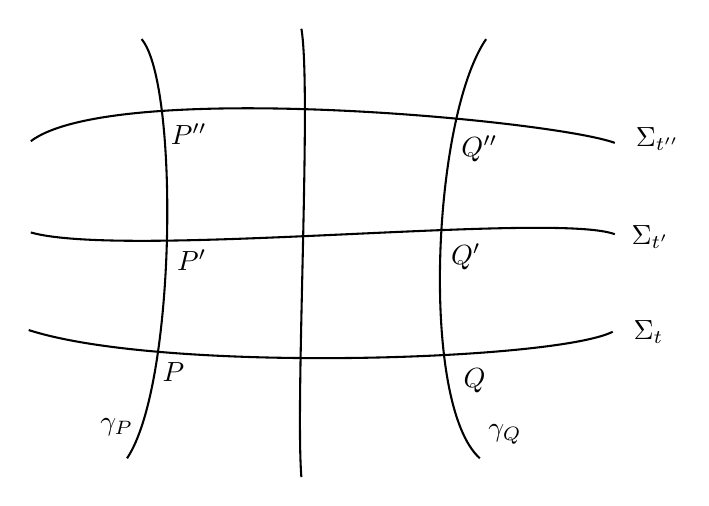
\begin{tikzpicture}[x=0.75pt,y=0.75pt,yscale=-1,xscale=1]
	%uncomment if require: \path (0,241); %set diagram left start at 0, and has height of 241
	
	%Curve Lines [id:da304112418408232] 
	\draw    (163,71) .. controls (203,41) and (414.37,60.82) .. (444.37,71.82) ;
	%Curve Lines [id:da26331590126988136] 
	\draw    (163,115) .. controls (209.37,127.82) and (414.37,104.82) .. (444.37,115.82) ;
	%Curve Lines [id:da04277550576726985] 
	\draw    (162,162) .. controls (226.37,182.82) and (415.37,176.82) .. (443.37,162.82) ;
	%Curve Lines [id:da5484171208567559] 
	\draw    (216.37,21.82) .. controls (234.37,42.82) and (233.37,187.82) .. (209.37,223.82) ;
	%Curve Lines [id:da16753899204609457] 
	\draw    (293.37,16.82) .. controls (298.37,45.82) and (290.37,195.82) .. (293.37,232.82) ;
	%Curve Lines [id:da24024484136290303] 
	\draw    (382.37,21.82) .. controls (356.37,59.82) and (350.37,197.82) .. (379.37,223.82) ;
	
	% Text Node
	\draw (195,203) node [anchor=north west][inner sep=0.75pt]    {$\gamma _{P}$};
	% Text Node
	\draw (382,206) node [anchor=north west][inner sep=0.75pt]    {$\gamma _{Q}$};
	% Text Node
	\draw (370,179) node [anchor=north west][inner sep=0.75pt]    {$Q$};
	% Text Node
	\draw (364,119) node [anchor=north west][inner sep=0.75pt]    {$Q'$};
	% Text Node
	\draw (369,67) node [anchor=north west][inner sep=0.75pt]    {$Q''$};
	% Text Node
	\draw (225,176) node [anchor=north west][inner sep=0.75pt]    {$P$};
	% Text Node
	\draw (232,122) node [anchor=north west][inner sep=0.75pt]    {$P'$};
	% Text Node
	\draw (229,61) node [anchor=north west][inner sep=0.75pt]    {$P''$};
	% Text Node
	\draw (453,63) node [anchor=north west][inner sep=0.75pt]    {$\Sigma _{t''}$};
	% Text Node
	\draw (451,110) node [anchor=north west][inner sep=0.75pt]    {$\Sigma _{t'}$};
	% Text Node
	\draw (452,156) node [anchor=north west][inner sep=0.75pt]    {$\Sigma _{t}$};
	
	
\end{tikzpicture}